\subsection{可和测度族的定义}

设 \((\lambda_{\alpha})_{\alpha \in \mathrm{A}}\) 是局部紧空间 \(X\) 上的一个正测度族；如果族 \((\lambda_{\alpha})_{\alpha \in \mathrm{A}}\) 在向量空间 \(\mathcal{M}(X)\) （\(X\) 上的实测度所成，赋以淡拓扑；GT, III, §5 第 1 号）中是可和的，就称它是可和测度族。这等于说，对每个函数 \(f \in \mathcal{H}(X)\) ，数族 \(\lambda_{\alpha}(f)\) 在 \(\mathbf{R}\) 中可和。因为这一条件显然是必要的；反之，若它满足，则线性形式 \(f \mapsto \sum_{\alpha \in \mathrm{A}} \lambda_{\alpha}(f)\) （\(\mathcal{H}(X)\) 上的）是正的，从而是一个正测度 \(\nu\) （第三章，§1 第 5 号定理 1），且可立即验证，族 \((\lambda_{\alpha})\) 的有限部分和淡收敛于 \(\nu\) （关于 \(A\) 的有限子集所成之集的截口滤子；GT, III, §5 第 1 号定义 1）。

由于 \(\mathcal{H}(\mathrm{X})\) 的每个元素都是 \(\mathcal{H}_{+}(\mathrm{X})\) 的两个元素之差，族 \((\lambda_{\alpha})\) 可和必须且只须

\[
\sum_ {\alpha \in A} \lambda_ {\alpha} (f) <   + \infty\tag{1}
\]

对每个函数 \(f \in \mathcal{K}_{+}(X)\) 。此条件也等价于下述条件：

\[
\sum_ {\alpha \in \mathrm{A}} \lambda_ {\alpha} (\mathrm{K}) <   + \infty\tag{2}
\]

对每个紧集 \(\mathrm{K} \subset \mathrm{X}\) 。

因为 (2) 蕴含 (1)，这是由于 \(f \leqslant \|f\| \cdot \varphi_{\mathrm{S}}\) ，其中 S 表示 \(f\) 的紧支集。反之，若 K 是紧集，则存在函数 \(f \in \mathcal{K}_{+}(\mathbf{X})\) 使 \(\varphi_{\mathrm{K}} \leqslant f\) （第三章，§1 第 2 号引理 1），由此 (1) 蕴含 (2)。

注记. --- 1) 立即可见，当族 \((\lambda_{\alpha})_{\alpha \in A}\) 可和时，它的和是 \(\mathcal{M}_{+}(X)\) 中有限部分和 \(\sum_{\alpha \in J} \lambda_{\alpha}\) 的上确界，其中 \(J\) 取遍 \(A\) 的有限子集所成之集。

\pandocbounded{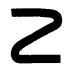
\includegraphics[keepaspectratio]{images/part002_9de8d58d.jpg}}

\begin{enumerate}
\def\labelenumi{\arabic{enumi})}
\setcounter{enumi}{1}
\tightlist
\item
  设 \((\theta_{\alpha})_{\alpha\in\mathbb{A}}\) 是 X 上的一个复测度族；就称族 \((\theta_{\alpha})\) 为可和的，如果正测度族 \((|\theta_{\alpha}|)\) 可和；族 \((\theta_{\alpha})\) 在赋以淡拓扑的向量空间 \(\mathcal{M}(X;\mathbf{C})\) 中可和并不足以保证这一点（参看习题 3）。
\end{enumerate}

